% =============================================================================
% Бүлэг 5: Туршилтын системийн хэрэгжүүлэлт
% =============================================================================

\chapter{Туршилтын системийн хэрэгжүүлэлт}
\label{ch:system}
\pagecolor{white}

Энэ бүлэгт санал болгосон дамжлагыг хэрэгжүүлсэн туршилтын системийг алхам бүрээр, мөн түүнийг үүлэн орчинд ажиллуулах,
хянах арга, судалгааны хэрэгслийг тайлбарлана.

\section{Системийн ерөнхий бүтэц}
\label{sec:sys-structure}

Систем нь Python (≥ 3.10) дээрх \tsql{mn\_text2sql} багц (85 модуль, ~17 500 мөр), YAML тохиргоо, bash ба notebook
скриптээс бүрдэнэ (Хүснэгт~\ref{tab:packages}). Бүх үйлдэл нэг \tsql{t2s} командын мөрийн хэрэгслээр хийгдэнэ
(\tsql{t2s db-build}, \tsql{index-build}, \tsql{eval}, \tsql{reselect}, \tsql{translate}, \tsql{flow-ui} г.м.,
Хавсралт~\ref{app:commands}; файлын бүтэц Хавсралт~\ref{app:files}).
Нэгжийн ба интеграцийн 100 гаруй тест (pytest) бий.

\begin{table}[H]
\centering\small
\caption{Кодын бүтэц}
\label{tab:packages}
\begin{tabularx}{\textwidth}{p{3.0cm}X}
\toprule
Дэд багц & Үүрэг \\
\midrule
\tsql{pipeline} & Шалгах, орчуулах, хайх, үүсгэх, диалект хөрвүүлэлт, засвар, санал хураалт \\
\tsql{retrieval}, \tsql{knowledge} & BM25 ба BGE-M3 индекс, schema linking, мэдлэгийн сан \\
\tsql{llm} & vLLM / OpenAI-тэй нийцтэй клиент, тестийн хуурамч загвар \\
\tsql{security} & SQL хамгаалалт (sqlglot), хориотой функц, injection тест \\
\tsql{db}, \tsql{datagen} & Өгөгдлийн сан, синтетик өгөгдөл, test-suite хуулбар \\
\tsql{eval}, \tsql{training} & Үнэлгээ, McNemar, GPU-гүй дахин сонголт; орчуулга, rejection sampling, SFT/QLoRA \\
\tsql{service} & FastAPI үйлчилгээ, Text2SQL Studio \\
\bottomrule
\end{tabularx}
\end{table}

\section{Асуулт хүлээн авах ба шалгах}
\label{sec:sys-intake}

Латин галигаар бичсэн асуултыг кирилл рүү хөрвүүлнэ (үгийн нарийвчлал 89.1\%-иас 94.8\% болгож сайжруулсан). Хувийн
мэдээлэл (регистр, утас, хаяг) асуусан, өгөгдөл өөрчлөх хүсэлттэй асуултаас дүрмээр татгалзана. Татгалзахаас бусад
шийдвэрийг загварт үлдээв: хэт идэвхтэй дүрэм хариулах боломжтой асуултыг алддаг нь туршилтаар ажиглагдсан.

\section{Асуултыг орчуулах}
\label{sec:sys-translate}

Монгол асуултыг Qwen3.5-9B-ээр англи руу орчуулна. DB-д байгаа утгыг \tsql{[V1]} маягийн маскаар хамгаалж, орчуулгын
дараа сэргээнэ; мэдлэгийн сангийн нэр томьёоны орчуулгыг зааварт нэмнэ (T2). Орчуулгын үр дүнг кэшлэж, ижил асуултыг
дахин орчуулахгүй.

\section{Мэдлэг хайх ба prompt угсрах}
\label{sec:sys-rag}

Дөрвөн индексээс хайна: (1) хүснэгт, баганын монгол тайлбар, синоним, enum кодын нэр; (2) текст баганын утга; (3)
байгууллагын нэр томьёо ба каноник SQL; (4) жишээ асуулт ба SQL (4 жишээ). Олдсон мэдлэг DDL-ийн comment ба асуултын өмнөх
evidence хэсэгт орж, Arctic-ийн сургалтын протоколын prompt угсрагдана.

\section{SQL үүсгэх, засах ба сонгох}
\label{sec:sys-generate}

Загвар SQLite-аар бичсэн SQL-ийг sqlglot-оор PostgreSQL руу хөрвүүлнэ. Boolean харьцуулалт (\tsql{= 1} → \tsql{= TRUE}),
код ↔ нэр, огнооны \tsql{LIKE} зэрэг жижиг алдааг дүрмээр засна. Гүйцэтгэлийн алдаа гарвал алдааны мессежээр 2 удаа хүртэл
засуулна (E1). Sampling-аар 8 хувилбар үүсгэж, гүйцэтгэлийн үр дүнгийн hash-аар санал хураана (E2); хоосон, бүгд NULL,
DB-д байхгүй текст утгатай хувилбарыг хасна (E4f). Олонхын хувь $< 0.5$ бол хамгийн их санал авсан хоёр тайлбарыг
харуулж тодруулга асууна (E3c). Санал хураах функцийг Эх код~\ref{lst:vote}-д үзүүлэв.

\begin{lstlisting}[language=Python, basicstyle=\ttfamily\scriptsize, caption={Гүйцэтгэлийн үр дүнгээр санал хураах (\tsql{pipeline/orchestrator.py})}, label={lst:vote}]
@staticmethod
def vote(cands, use_filter=False):
    good = [c for c in cands if c.ok and c.result_hash]   # (*@алдаагүй, үр дүнтэй хувилбар@*)
    if not good:
        return cands[0], 0.0, False
    if use_filter:  # E4f: (*@хоосон/NULL, DB-д байхгүй утгатайг хасна@*)
        good = [c for c in good if not c.degenerate and not c.bad_literals] or good
    counts = Counter(c.result_hash for c in good)
    best_hash, best_n = max(counts.items(), key=lambda kv: (kv[1], -min(
        i for i, c in enumerate(cands) if c.result_hash == kv[0])))   # (*@тэнцвэл эхний хувилбар@*)
    chosen = next(c for c in good if c.result_hash == best_hash)
    conf = best_n / len(cands)                            # (*@итгэл = олонхын хувь@*)
    return chosen, conf, best_n == len(cands)
\end{lstlisting}

\textbf{Жишээ: нэг асуултын явц.} Dev-ийн A020 асуулт E2 тохиргоогоор дараах алхмаар боловсруулагдсан (бодит run-ийн бүртгэлээс):
\begin{enumerate}
  \item \textbf{Асуулт:} «Шийдвэр гаргасан түвшин бүрээр хүсэлтийг дунджаар хэдэн хоногт шийдвэрлэсэн бэ?»
  \item \textbf{Орчуулга:} «On average, how many days does it take to resolve requests at each decision-making level?»
  \item \textbf{Мэдлэг хайлт:} 6 хүснэгт (\tsql{loan\_applications}, \tsql{loans}, \tsql{customers} г.м.), 5 нэр томьёо
        (\tsql{approval\_rate}, \tsql{rejection\_rate} г.м.), 4 жишээ (AX16, AX19, AX15, PX16).
  \item \textbf{Санал хураалт:} 8 хувилбараас 5 нь ижил (зөв) үр дүнтэй, 3 нь өөр --- итгэл 0.625 ($\geq 0.5$ тул хариулна).
  \item \textbf{Эцсийн SQL} (зөв):
\end{enumerate}
\begin{lstlisting}[language=SQLmn, basicstyle=\ttfamily\scriptsize]
SELECT decision_level,
       ROUND(CAST(AVG(decided_date - submitted_date) AS DECIMAL), 2) AS avg_days_to_decide
FROM loan_applications
WHERE NOT decided_date IS NULL AND NOT submitted_date IS NULL
GROUP BY decision_level
\end{lstlisting}
Ганц үүсгэлттэй тохиргоо 8-аас 3 магадлалтайгаар буруу хувилбар сонгох байсныг санал хураалт зассан нь H4 → E2-ийн
ахицын механизмыг харуулж байна.

\section{Аюулгүй гүйцэтгэл ба аудит}
\label{sec:service}

SQL-ийг ганц \tsql{SELECT}/\tsql{WITH} эсэх, хориотой үйлдэл ба 35 гаруй функц (\tsql{pg\_sleep}, \tsql{dblink} г.м.),
зөвхөн \tsql{t2s} схемийн view, EXPLAIN-ийн өртгийн хязгаараар шалгана. Bot хэрэглэгч зөвхөн \tsql{SELECT} эрхтэй; холболт
бүр read-only транзакц, 20 секундийн timeout-той; мөрийн түвшний хамгаалалт (RLS) салбарын хэрэглэгчид зөвхөн өөрийн
салбарын мөрийг харуулна. FastAPI үйлчилгээ shadow, pilot, live горимтой; аудитын бүртгэлд асуулт ба SQL-ийг Fernet-ээр
шифрлэж 90 хоног хадгална. Аюулгүй байдлын тест 28 SQL халдлага, монгол ба латинаар бичсэн 56 prompt injection, RLS-ийг
шалгаж бүгд хаагдсан.

\section{Text2SQL Studio дээр дүрслэх}
\label{sec:studio}

Туршилтын тохиргоог ойлгомжтой харуулах, нэг асуулт дээр алхам бүрийн нөлөөг шууд харах вэб хэрэгслийг хөгжүүлэв
(Зураг~\ref{fig:studio}). Дамжлагын алхам бүр node болж (Drawflow), тохиргоо \tsql{config/flows.yaml}-д хадгалагдана.
Emulator-т асуулт асууж хариулт, хүснэгт, SQL-ийг харахад ажиллаж буй node анивчиж, алхам бүрийн хугацаа амьдаар гарна.
Debugger нь алхам бүрийн оролт гаралт, загварт очсон бүтэн prompt, хайлтаар олдсон мэдлэг оноотой, токены задаргааг
харуулна. Prompt-ыг үнэлгээнд ашигладаг \tsql{ask()}-тай ижил замаар угсардаг тул харагдах prompt бодит туршилтынхтай
ижил.

\begin{figure}[htbp]
\centering
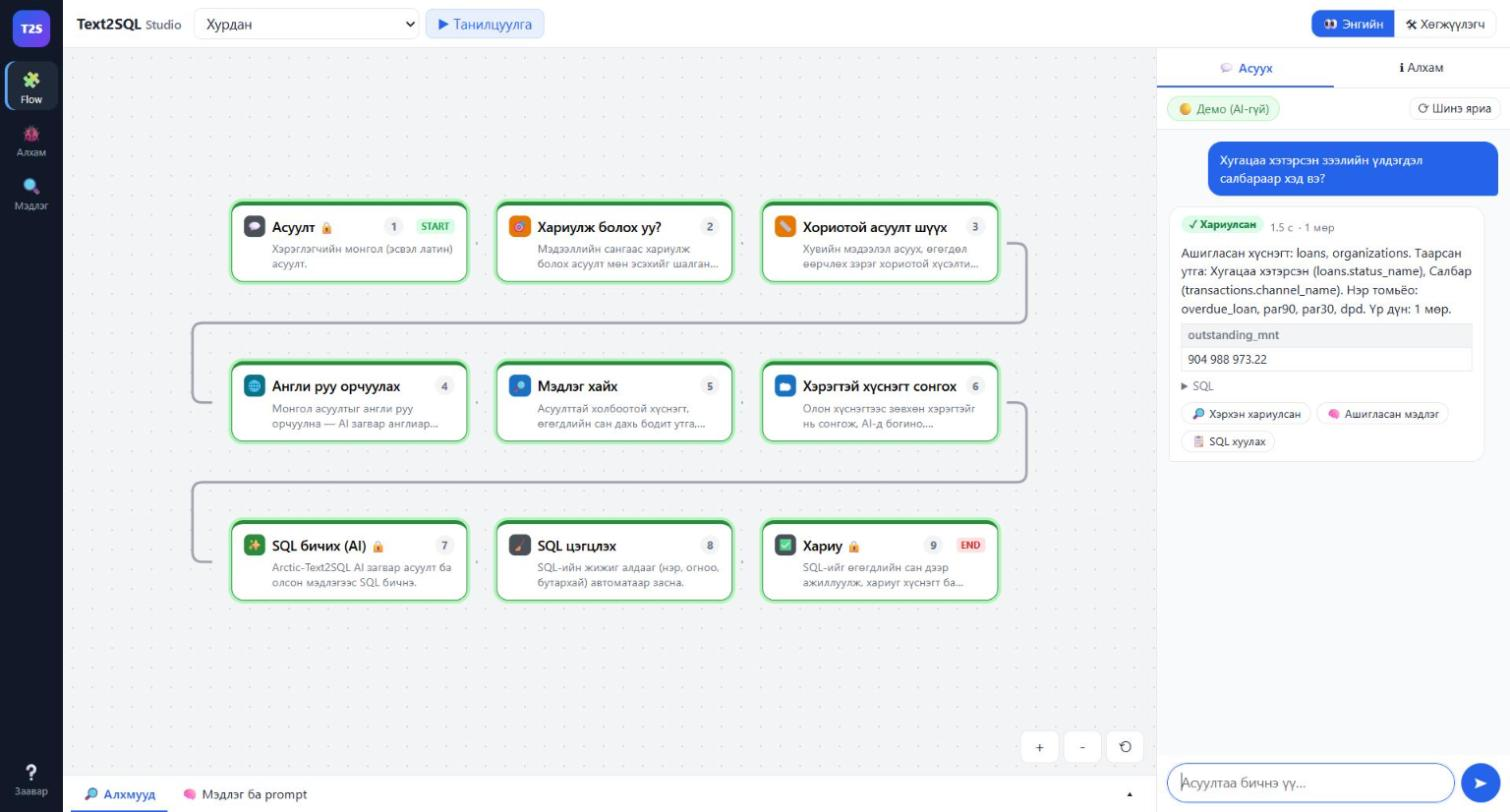
\includegraphics[width=0.92\textwidth]{Figures/studio.jpg}
\caption{Text2SQL Studio: дамжлагын алхмууд (зүүн), асуулт ба хариулт (баруун), демо горим}
\label{fig:studio}
\end{figure}

\section{Загварын үндсэн зарчмууд}
\label{sec:principles}

\begin{table}[H]
\centering\small
\caption{Системийн дизайны үндсэн зарчмууд}
\label{tab:principles}
\begin{tabularx}{\textwidth}{p{4.0cm}X}
\toprule
Зарчим & Хэрэгжилт \\
\midrule
Алхам бүр асааж унтрах & Тохиргооны нэг талбар = нэг алхам; 84 нэрлэсэн тохиргоо \\
Тогтмол мэдлэг жинд, өөрчлөгдөх мэдлэг RAG-д & SQL чадвар ба хэл --- сургалт; схем, нэр томьёо, утга --- хайлт \\
Буруу хариултаас татгалзах нь дээр & Дүрмээр татгалзах, итгэл багатай үед тодруулах \\
Өгөгдөл гадагш гарахгүй & Нээлттэй эхийн загвар, байгууллагын дотор нэг GPU \\
Давхар хамгаалалт & SQL шалгалт + DB-ийн эрх, RLS, read-only \\
Давтагдах байдал & Run бүрт үнэлгээний сан, DB, prompt, тохиргооны hash; ижил \tsql{t2s eval} команд \\
Тасалдлаас сэргэх & Kaggle-ийн 12 цагийн сесс: checkpoint ба үр дүнг дараагийн сесс үргэлжлүүлнэ \\
\bottomrule
\end{tabularx}
\end{table}

\textbf{Үүлэн орчин.} Өөрийн GPU сервергүй тул туршилтыг Kaggle notebook-оор ажиллуулав. Кодыг хувийн dataset болгон
байршуулж, notebook орчныг суулгаад \tsql{run\_plan\_l4.sh}-ийн үе шатыг (\tsql{STAGE=e2test | istage | train\_d3 | mt |
web}) гүйцэтгэнэ. Тохиргоог \tsql{config/kaggle\_overrides.env} файлаар өгч, өмнөх сессийн гаралтыг дараагийн сессийн
оролт болгоно.

\section{Системийн хязгаарууд ба цаашдын ажил}
\label{sec:sys-limits}

\begin{itemize}
  \item \textbf{Хурд.} 8 хувилбартай E2 T4 дээр асуулт бүрт ~3 минут зарцуулдаг (§\ref{sec:latency}); бодит хэрэглээнд
        нэг үүсгэлттэй I3t маягийн тохиргоо эсвэл илүү хүчтэй GPU шаардлагатай.
  \item \textbf{Kaggle вэб.} Kaggle дээр ажиллуулсан Studio-д эхний асуулт 9 минутаас удаан үргэлжилсэн; шалтгааныг
        оношлох зорилгоор лог ба амьд явцыг нэмсэн.
  \item \textbf{Нэг байгууллага.} Мэдлэгийн сан нэг схемд зориулагдсан; өөр байгууллагад шилжүүлэхэд дахин бэлтгэх
        шаардлагатай. Схем солигдоход тогтвортой байх сургалт (S1--S4) ба үнэлгээ (T-2, T-4) бэлэн болсон.
\end{itemize}

\section{Бүлгийн дүгнэлт}
\label{sec:ch6-summary}

Туршилтын систем нь асуулт шалгах, орчуулах, мэдлэг хайх, SQL үүсгэх, засах, сонгох, аюулгүй гүйцэтгэх алхмуудыг командын
мөрийн нэг хэрэгсэл болгон хэрэгжүүлж, үүлэн орчинд тасалдлаас сэргэдэг ажиллуулалт, давхаргатай аюулгүй байдал, туршилтыг
ил тод харуулах Text2SQL Studio-оос бүрдэнэ.
